% Modulo 1: Telescopios-Generalidades
% Objetivo: Proporcionar a los miembros del club la información fundamental de telescopios con énfasis en telescopios Newtonianos (reflectores), incluyendo historia, principios ópticos, ventajas y desventajas y aplicaciones básicas. 

\section{Introducción}

La palabra telescopio proviene del griego \foreignlanguage{greek}{τῆλε} (tēle, “lejos”) y \foreignlanguage{greek}{σκοπέω} (skopeō, “observar”); es decir, un instrumento utilizado para observar a lo lejos. Estos instrumentos ópticos permiten captar con mayor precisión y detalle una porción de la radiación electromagnética proveniente de cuerpos distantes.

Su invención y desarrollo han sido fundamentales para la observación y comprensión del universo. Gracias al telescopio, la humanidad ha podido explorar objetos cercanos como el Sol, la Luna, los planetas y sus satélites, así como estructuras mucho más lejanas como nebulosas, cúmulos estelares y galaxias remotas (fig.~\ref{fig:telescopio_antiguo}).

\begin{figure}[H]
	\centering
	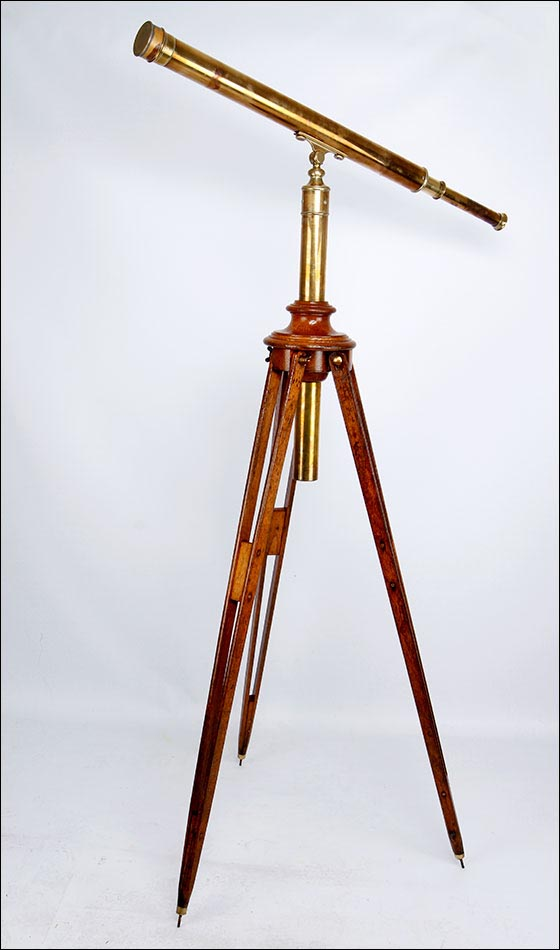
\includegraphics[width=0.6\textwidth]{images/telescopio_antiguo.jpg}
	\caption{Telescopio antiguo, aproximadamente de principios de 1800.}
	\label{fig:telescopio_antiguo}
\end{figure}

Históricamente, la primera patente de un telescopio refractor fue solicitada por Hans Lipperhey, un fabricante de lentes neerlandés. La idea de utilizar dos lentes en un instrumento óptico se difundió rápidamente por Europa, llegando al conocimiento de Galileo Galilei, quien construyó su propia versión y la utilizó para observar el cielo nocturno. Con ella logró visualizar objetos invisibles al ojo humano, como las lunas de Júpiter y estrellas ubicadas en regiones aparentemente “vacías” del cielo.

La versión de Galileo permitía un aumento de hasta 8 veces. Si bien sus primeros usos fueron de tipo militar —otorgando ventaja táctica al enemigo—, Galileo también aprovechó su invento para fines científicos y astronómicos.

Gracias a estas observaciones, Galileo obtuvo evidencias a favor de la teoría copernicana, la cual ubicaba al Sol en el centro del sistema, en oposición a la teoría geocéntrica dominante que situaba a la Tierra como el centro del universo.

\begin{figure}[H]
	\centering
	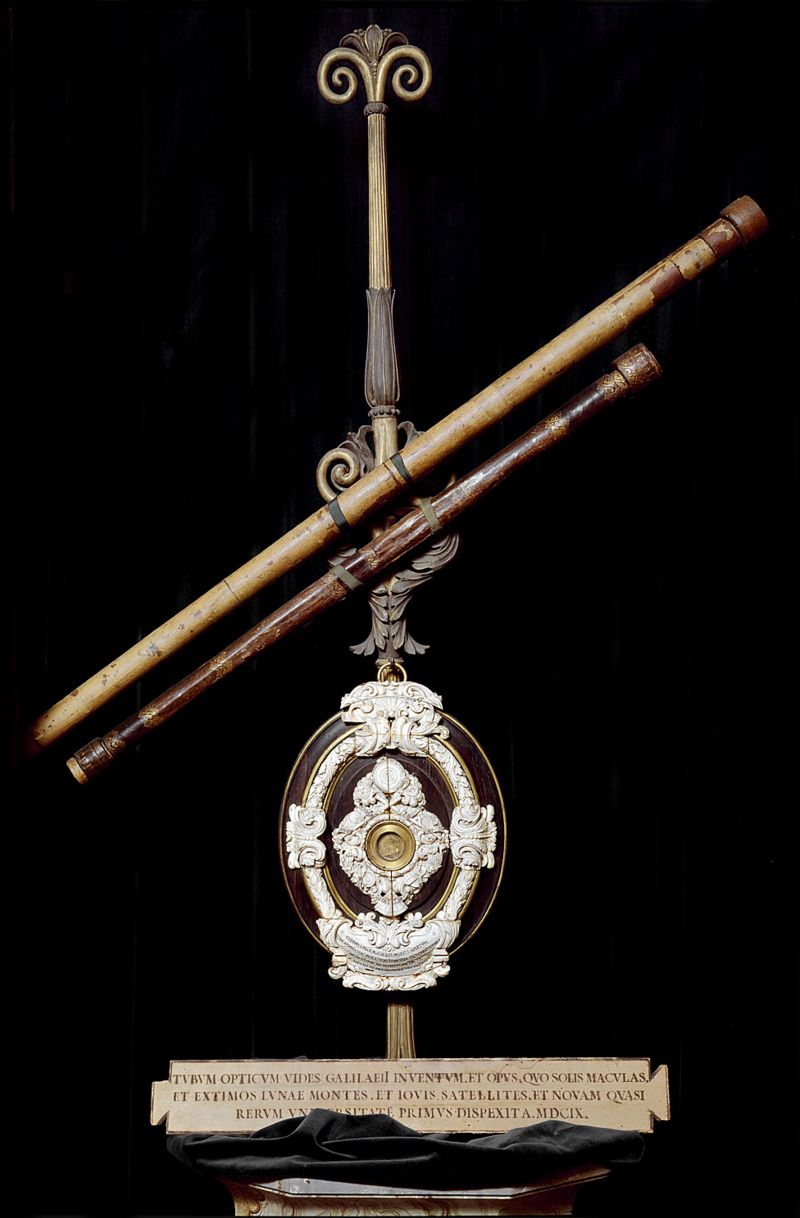
\includegraphics[width=0.6\textwidth]{images/telescopio_galileo.jpg}
	\caption{Versión modificada del telescopio tradicional construida por Galileo, optimizada para captar objetos lejanos.}
	\label{fig:telescopio_patente_galileo}
\end{figure}

El término \textbf{telescopio} abarca una amplia variedad de dispositivos: radiotelescopios, telescopios infrarrojos y ultravioletas, así como \textbf{telescopios ópticos}. En este documento nos enfocaremos en estos últimos, por ser los más comunes y accesibles, ideales para introducirse en el mundo de la observación astronómica.

Esta guía forma parte del minicurso organizado por la Comisión de Creación de Telescopios del Capítulo de Óptica de Yachay Tech, realizado en abril de 2024.

\subsection*{Breve historia del telescopio}

El registro más antiguo del uso de un telescopio refractor corresponde a una patente solicitada por Hans Lipperhey en los Países Bajos, en el siglo XVII. Aunque no se le otorgó la patente, su diseño se popularizó rápidamente por toda Europa. En 1609, Galileo Galilei lo utilizó con fines astronómicos para observar el cielo, marcando un hito en la historia de la ciencia. Sus observaciones respaldaban la teoría heliocéntrica y contradecían la cosmología geocéntrica dominante, según la cual la Tierra ocupaba el centro del universo, con los planetas, la Luna y las estrellas girando alrededor de ella.

Galileo no sólo registró sus observaciones, sino que también las ilustró cuidadosamente (fig.~\ref{fig:ilustracion_luna_galileo_1610}). A esta revolución científica se sumó Johannes Kepler, quien perfeccionó el diseño de Galileo mejorando el campo de visión —aunque invirtiendo la imagen—, sentando las bases de los telescopios astronómicos modernos.

\begin{figure}[H]
	\centering
	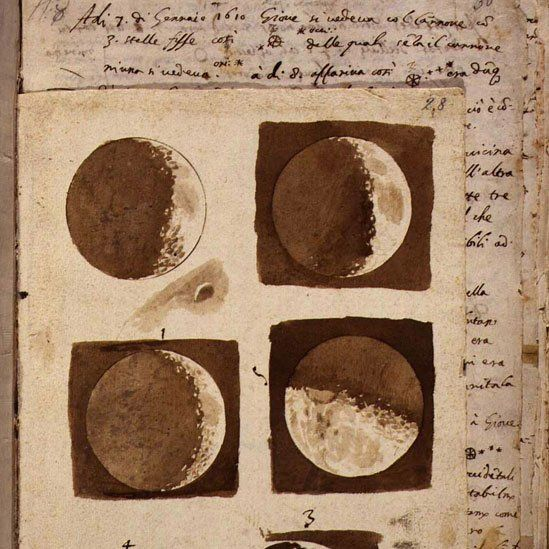
\includegraphics[width=0.6\textwidth]{images/ilustracion_galileo.jpg}
	\caption{Ilustración de la Luna realizada por Galileo Galilei en 1610, incluida en su obra *Sidereus Nuncius*.}
	\label{fig:ilustracion_luna_galileo_1610}
\end{figure}

Con el tiempo, se comenzó a experimentar con espejos en lugar de lentes para captar la luz, lo que ayudó a evitar ciertos problemas ópticos recurrentes. En 1668, Isaac Newton construyó el primer telescopio reflector funcional, hoy conocido como telescopio reflector newtoniano (fig.~\ref{fig:telescopio_reflector_newotoniano}). Este diseño usaba un espejo cóncavo hecho de una aleación de cobre y estaño pulido, en lugar de lentes, lo que permitía evitar aberraciones cromáticas.

Durante más de un siglo, los telescopios refractores evolucionaron lentamente, hasta que en 1730 se introdujeron lentes acromáticas, lo que mejoró considerablemente la calidad de imagen. Los primeros telescopios reflectores, por su parte, enfrentaban el problema de pérdida de brillo debido a la oxidación de los espejos metálicos (fig.~\ref{fig:espejo_metalico_especulum}). Este inconveniente comenzó a resolverse en la década de 1850 con el uso de espejos de vidrio recubiertos, y más tarde, en 1932, con la implementación de espejos aluminizados.

%\begin{figure}[H]
%	\centering
%	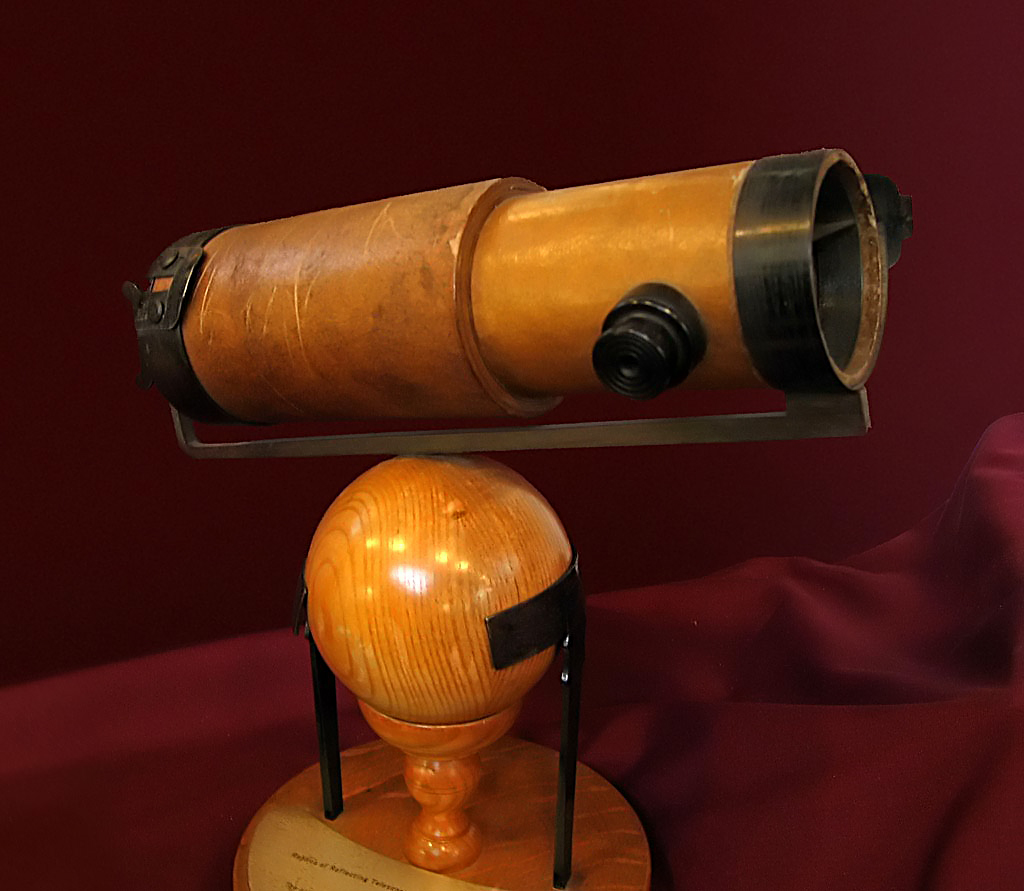
\includegraphics[width=0.6\textwidth]{newton_reflector_telescopio.jpg}
%	\caption{Réplica del primer telescopio reflector registrado por Isaac Newton ante la Royal Society en 1672.}
%	\label{fig:telescopio_reflector_newotoniano}
%	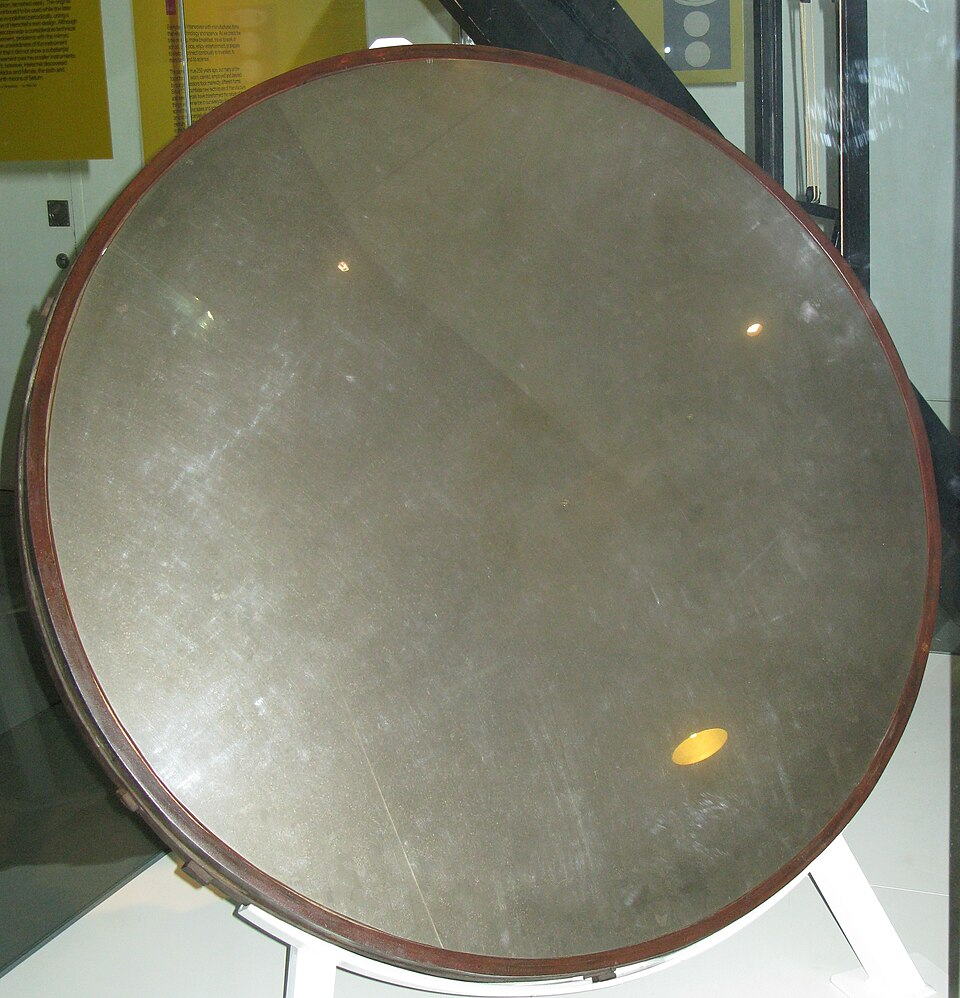
\includegraphics[width=0.6\textwidth]{speculum_mirror_metal.jpg}
%	\caption{Espejo metálico de 1.2 m de diámetro para un telescopio de 40 pies.}
%	\label{fig:espejo_metalico_especulum}
%\end{figure}

A mediados del siglo XX, los telescopios refractores más grandes alcanzaban aperturas de aproximadamente $1\,\mathrm{m}$ (39 pulgadas), mientras que los reflectores superaban los $10\,\mathrm{m}$ (33 pies). Actualmente, se están construyendo telescopios aún más grandes, con aperturas de entre 30 y 40 metros, muchos de ellos situados en órbita para evitar las distorsiones de la atmósfera terrestre.

Aun así, los telescopios ópticos terrestres siguen siendo herramientas científicas de gran valor, gracias a las tecnologías modernas que permiten desarrollar soluciones ópticas adaptativas, de bajo costo y gran impacto en la investigación astronómica. Además, los nuevos algoritmos de procesamiento de imágenes y corrección de aberraciones proporcionan un marco teórico y práctico para el diseño de instrumentos ópticos avanzados (figs.~\ref{fig:gran_telescopio_canarias}, \ref{fig:gmt_chile}).

\begin{figure}[H]
	\centering
	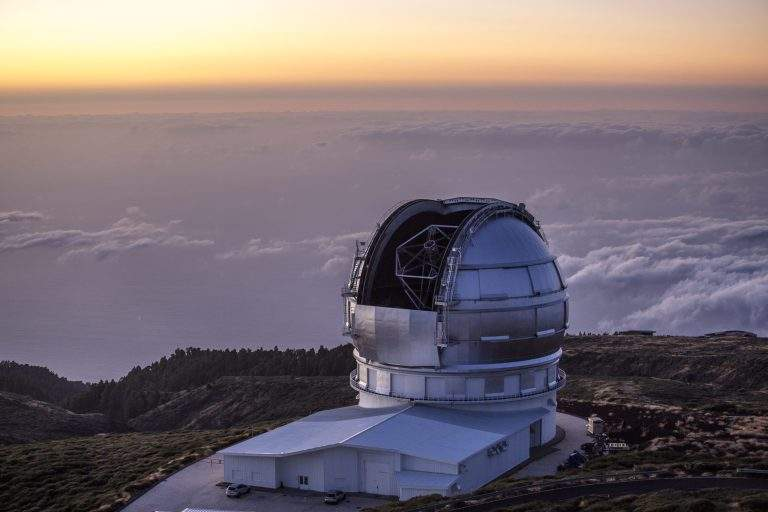
\includegraphics[width=0.6\textwidth]{images/gran_telescopio_canarias.jpg}
	\caption{Gran Telescopio de Canarias (GTC). Telescopio reflector con un espejo principal de 10.4 m de diámetro, compuesto por 36 segmentos hexagonales.}
	\label{fig:gran_telescopio_canarias}
	
	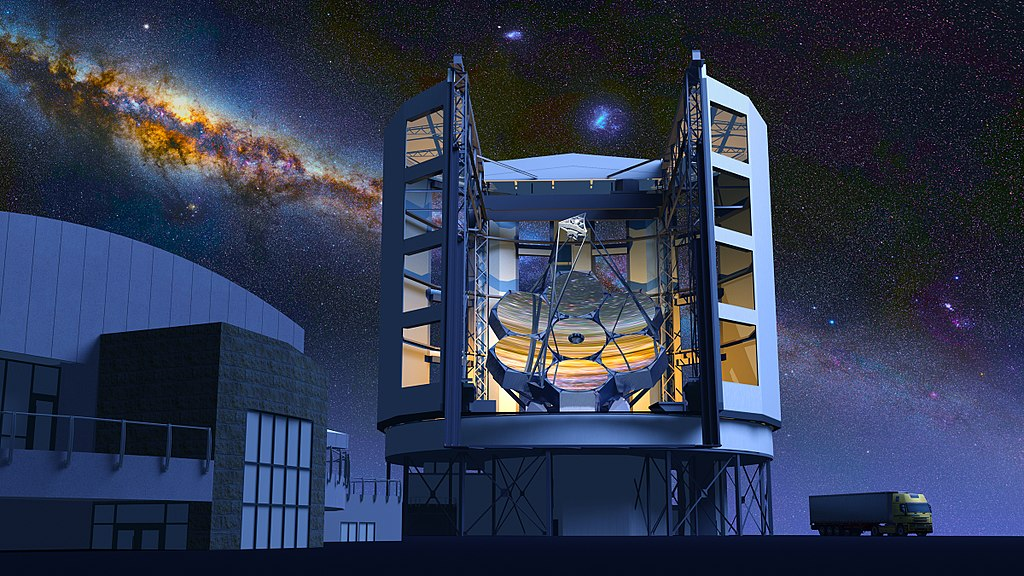
\includegraphics[width=0.6\textwidth]{images/giant_magallan_telescope.jpg}
	\caption{Giant Magellan Telescope (GMT), uno de los tres telescopios más grandes actualmente en construcción, ubicado en el desierto de Atacama, Chile.}
	\label{fig:gmt_chile}
\end{figure}


\section{Principios Ópticos Fundamentales}

\subsection*{La luz y su velocidad}

La luz, tal como la percibimos, corresponde a una fracción del espectro electromagnético que puede ser detectada por nuestro sistema visual. Su definición, en términos prácticos, está íntimamente relacionada con la respuesta fisiológica y psicológica del sistema ojo-cerebro frente a estímulos dentro del rango de la luz visible, que abarca longitudes de onda entre $400$ y $700\,\mathrm{nm}$.

Por ejemplo, una mezcla de luz roja y verde es interpretada por nuestro sistema visual como luz amarilla, aunque no exista radiación electromagnética en la longitud de onda correspondiente al amarillo. Este fenómeno se conoce como \textit{mezcla aditiva de colores}, y es una propiedad emergente del procesamiento neuronal de la luz, más que una característica física de la radiación.

\vspace{0.3cm}
% FIGURA sugerida: diagrama con el espectro visible y un círculo de mezcla RGB

\subsection*{Historia de la medición de la velocidad de la luz}

Desde hace siglos, el ser humano ha intentado determinar si la luz posee una velocidad finita o si se propaga instantáneamente. Con el desarrollo de los telescopios comenzaron a realizarse los primeros experimentos.

\paragraph{Galileo Galilei (siglo XVII):} Galileo intentó medir la velocidad de la luz con ayuda de un asistente. Cada uno portaba una linterna, y se situaban a unos tres kilómetros de distancia. Galileo destapaba su linterna y, al ver la luz, el asistente debía destapar la suya en respuesta. Galileo cronometraba el tiempo entre su acción inicial y la percepción del reflejo.

Aunque ingenioso, el experimento no tuvo éxito. Hoy sabemos que la luz recorre esa distancia en aproximadamente $10^{-5}$ segundos, un intervalo imposible de medir con los instrumentos disponibles en la época. Además, el tiempo de reacción humana introducía un margen de error considerable.

\vspace{0.3cm}
% ILUSTRACIÓN sugerida: recreación simple del experimento con linternas

\paragraph{Ole Rømer (1675):} El astrónomo danés Ole Rømer estudió durante varios años los eclipses de Io, una de las lunas de Júpiter. Observó que el tiempo entre eclipses variaba dependiendo de la posición relativa entre la Tierra y Júpiter: cuando la Tierra se alejaba, los eclipses parecían retrasarse.

Rømer concluyó que la luz no se propagaba instantáneamente, sino que tardaba un tiempo finito en recorrer la distancia. Su trabajo representó la primera demostración experimental indirecta de que la luz tiene velocidad finita.

\vspace{0.3cm}
% ILUSTRACIÓN sugerida: esquema Tierra-Júpiter con Io mostrando trayectos de luz más largos/cortos

\paragraph{James Bradley (1728):} El físico británico James Bradley utilizó un telescopio para observar un fenómeno conocido como aberración estelar. Detectó un desplazamiento cíclico de toda la esfera celeste a lo largo del año, el cual solo podía explicarse considerando la velocidad orbital de la Tierra y una velocidad finita de la luz.

Su cálculo fue notablemente preciso para la época, estimando un valor cercano a $301,000\,\mathrm{km/s}$.

\paragraph{Hippolyte Fizeau (1849):} El físico francés diseñó un experimento de laboratorio utilizando una rueda dentada giratoria y un haz de luz dirigido a un espejo situado a unos 8 km. Cuando la rueda alcanzaba cierta velocidad, el haz de luz reflejado quedaba bloqueado por el siguiente diente, permitiendo calcular el tiempo de viaje de la luz.

Este fue el primer experimento exitoso para medir la velocidad de la luz sin necesidad de observaciones astronómicas.

\paragraph{Albert A. Michelson (1879):} Michelson perfeccionó el método de Fizeau utilizando un espejo giratorio de alta precisión. El haz de luz era reflejado hacia un espejo distante y, al regresar, su desviación permitía calcular con precisión la velocidad de la luz. Este método se convirtió en uno de los más confiables del siglo XIX y le valió el Premio Nobel de Física en 1907.

\vspace{0.3cm}
% FIGURAS sugeridas: diagrama de rueda dentada de Fizeau y espejo giratorio de Michelson

\subsection*{Relación con las constantes electromagnéticas}

En la actualidad, uno de los métodos más exactos para conocer la velocidad de la luz se basa en las constantes fundamentales del electromagnetismo. La relación está dada por:

\[
c = \frac{1}{\sqrt{\epsilon_0 \mu_0}}
\]

Donde:
\begin{itemize}
	\item $\epsilon_0$ es la permitividad eléctrica del vacío ($8.854 \times 10^{-12}\, \text{F/m}$),
	\item $\mu_0$ es la permeabilidad magnética del vacío ($4\pi \times 10^{-7}\, \text{N/A}^2$).
\end{itemize}

Esta expresión, derivada de las ecuaciones de Maxwell, describe cómo los campos eléctricos y magnéticos se propagan en el vacío. Como la luz es una onda electromagnética, su velocidad está determinada por estas constantes, lo cual demuestra que su propagación es finita y constante.

\begin{mybox}[blue]{Velocidad de la luz en el vacío}[colbacktitle=blue!30!white, coltitle=black]
	$c = 299\,792\,458 \, \text{m/s} \approx 3\cdot10^8 \text{m/s}$ 
\end{mybox}

\vspace{0.3cm}
% FIGURA sugerida: resumen visual con ecuación, valor de c, y conexión con unidades SI


\section*{Propagación de la luz}

La propagación de la luz, al tratarse de una oscilación del campo electromagnético, está regida por la ecuación de onda. No obstante, mucho antes de que Maxwell desarrollara la teoría del electromagnetismo, la propagación de la luz ya había sido descrita empíricamente mediante dos principios fundamentales: el \textbf{Principio de Huygens} y \textbf{el Principio de Fermat}.

El principio de Huygens, propuesto por el físico holandés Christiaan Huygens en el siglo XVII, describe el comportamiento de los frentes de onda de forma geométrica:

\begin{mybox}[green]{Principio de Huygens}[colbacktitle=blue!30!white, coltitle=black]
	Cada punto de un frente de onda primario actúa como foco, o fuente, de ondas esféricas secundarias que se propagan con la misma velocidad y frecuencia que la onda original. El nuevo frente de onda, al cabo de un intervalo de tiempo, es la envolvente de estas ondas secundarias.
\end{mybox}

Por otro lado, el principio de Fermat, basado en una idea geométrica y variacional, establece:

\begin{mybox}[green]{Principio de Fermat}[colbacktitle=blue!30!white, coltitle=black]
	La trayectoria que sigue la luz al pasar de un punto \textbf{A} a un punto \textbf{B} es aquella en la que el tiempo de recorrido es mínimo. Es decir, la luz tiende a seguir el camino óptico más rápido.
\end{mybox}

\vspace{0.3cm}
% FIGURA SUGERIDA: Comparación visual de Huygens y Fermat con una superficie separadora aire-vidrio

Estos principios no solo son compatibles, sino que se complementan. El primero ofrece una visión geométrica local, útil para explicar fenómenos como la difracción, mientras que el segundo permite deducir leyes globales como la de la refracción.

Ambos principios han sido herramientas esenciales en la óptica geométrica. Por ejemplo, el principio de Fermat permite derivar directamente la ley de Snell al analizar el cambio de trayectoria de la luz cuando atraviesa medios con diferente índice de refracción. En cambio, el principio de Huygens resulta fundamental para interpretar cómo se propaga una onda al encontrarse con una rendija o un obstáculo, fenómeno conocido como difracción.

Además, con el desarrollo posterior de la teoría ondulatoria y la óptica física, se comprendió que estas aproximaciones, aunque simples, son consistentes con la naturaleza ondulatoria de la luz y siguen siendo válidas en muchos contextos experimentales. Especialmente en situaciones donde las longitudes de onda son pequeñas en comparación con los objetos que la luz encuentra en su trayectoria, lo que permite aplicar la óptica geométrica de forma efectiva.

\vspace{0.3cm}
% ILUSTRACIÓN SUGERIDA: Visualización de rayos con cambio de medio + frentes de onda + interferencia

Por eso, al estudiar telescopios o cualquier sistema óptico, estos principios permiten anticipar cómo se comportará la luz al interactuar con lentes, espejos o incluso con la atmósfera. Aunque hoy contamos con modelos matemáticos más completos, estas ideas siguen siendo base de todo diseño óptico.


\section{Reflexión y Refracción}

La velocidad de la luz en medios transparentes como el aire, el agua o el vidrio es menor que su velocidad en el vacío. Esta diferencia da lugar a un parámetro óptico llamado \textbf{índice de refracción}, el cual se define como:

\begin{mybox}[blue]{Índice de refracción}[colbacktitle=blue!30!white, coltitle=black]
	$n = \frac{c}{v}$
\end{mybox}

donde:
\begin{itemize}
	\item $c$ es la velocidad de la luz en el vacío,
	\item $v$ es la velocidad de la luz en el medio considerado.
\end{itemize}

Cuando un rayo de luz incide sobre la interfaz entre dos medios con diferente índice de refracción (por ejemplo, aire y vidrio), una parte de la energía se refleja y otra parte penetra en el segundo medio, cambiando de dirección. Este fenómeno se conoce como \textbf{refracción}.

\begin{figure}[H]		
	\centering
	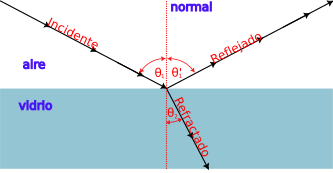
\includegraphics[width=0.6\textwidth]{images/refraction_reflection.png}
	\caption{El ángulo de reflexión es igual al ángulo de incidencia. El ángulo de refracción $\theta_2$ depende de la relación entre las velocidades de propagación en ambos medios.}
	\label{fig:refraccón_reflexión_planos}
\end{figure} 

En la figura \ref{fig:refraccón_reflexión_planos}, se observa un rayo de luz incidente sobre la superficie de un vidrio. El ángulo $\theta_1$ entre el rayo incidente y la normal se denomina \textbf{ángulo de incidencia}, y el plano definido por ambos se llama \textbf{plano de incidencia}.

El rayo reflejado se encuentra en el mismo plano y forma un ángulo igual con la normal, lo cual se expresa con la \textbf{ley de la reflexión}:

\begin{mybox}[blue]{Ley de la reflexión}[colbacktitle=blue!30!white, coltitle=black]
	$\theta'_1 = \theta_1$
\end{mybox}

Por otro lado, el rayo que entra al segundo medio (el rayo \textbf{refractado}) cambia de dirección debido al cambio de velocidad de propagación. La relación entre los ángulos y las velocidades en cada medio se expresa como:

\begin{equation}
	\frac{1}{v_1} \sin(\theta_1) = \frac{1}{v_2} \sin(\theta_2)
	\label{eq:refraccion_dos_medios}
\end{equation}

Si sustituimos las velocidades por sus respectivas expresiones en términos del índice de refracción ($v = c/n$), obtenemos la conocida \textbf{ley de Snell}:

\begin{mybox}[blue]{Ley de Snell de la refracción}[colbacktitle=blue!30!white, coltitle=black]
	$n_1 \sin(\theta_1) = n_2 \sin(\theta_2)$
\end{mybox} 

\subsection{Mecanismos físicos de la reflexión y la refracción}

A nivel microscópico, la reflexión y la refracción pueden entenderse como fenómenos de interacción entre la luz y los átomos del medio. Cuando un rayo de luz incide sobre una superficie, sus campos eléctricos hacen oscilar las cargas (principalmente electrones) en los átomos del material. Estas oscilaciones inducidas producen una nueva radiación: la luz es absorbida y reemitida por los átomos.

En la reflexión, parte de las ondas reemitidas se propagan en dirección opuesta al haz de luz incidente. Debido a interferencias constructivas, estas ondas se refuerzan en una dirección bien definida, formando el rayo reflejado.

En la refracción, la luz reemitida hacia adelante también sufre interferencia constructiva, pero en una dirección distinta a la original. El resultado neto es un cambio en la dirección de propagación, determinado por la diferencia de velocidades de fase en cada medio.

\subsection*{Reflexión Especular y Difusa}

La reflexión especular ocurre en superficies suaves y lisas. Como se muestra en la figura \ref{fig:ref_especular_difusa}, los rayos de luz provenientes del objeto $P$ se reflejan en el espejo formando una imagen como si provinieran del punto $P'$, conocida como la \textbf{imagen virtual} del punto $P$.

Por otro lado, la reflexión difusa ocurre cuando la superficie es rugosa, es decir, los rayos provenientes de un punto se reflejan en múltiples direcciones y no divergen desde un único punto.

\begin{figure}[H]
	\centering
	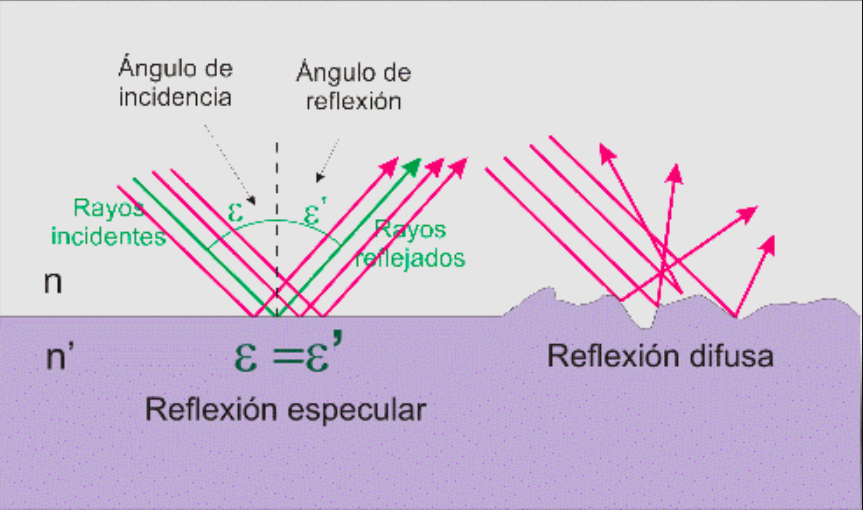
\includegraphics[width=0.6\textheight]{ref_especular_difusa.png}
	\caption{Reflexión especular y difusa.}
	\label{fig:ref_especular_difusa}
\end{figure}

\subsection*{Dispersión}

El índice de refracción de un material depende ligeramente de la longitud de onda de la luz incidente. Para la mayoría de los materiales, $n$ disminuye a medida que aumenta la longitud de onda. Esta dependencia se conoce como \textbf{dispersión}.

\begin{figure}[H]
	\centering
	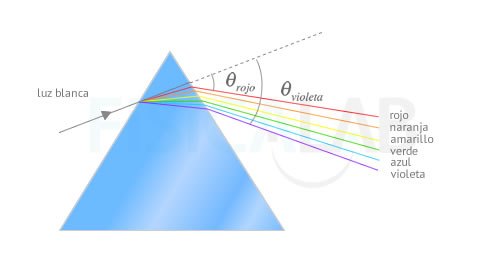
\includegraphics[width=0.6\textwidth]{images/descomposicion_luz.jpg}
	\caption{Descomposición de la luz blanca al atravesar un prisma.}
	\label{fig:dispersion_prisma_luz}
\end{figure}

\subsection{Reflexión y Espejos}

\subsubsection*{Espejos Planos}

Los espejos planos son los más comunes. En la figura \ref{fig:esplejos_planos} se ilustran dos rayos que provienen de los extremos de una botella (en realidad van en todas las direcciones), pero son los que entran en el ojo. Los rayos reflejados parecen provenir de un punto detrás del espejo: la \textbf{imagen virtual}. Siempre que un objeto esté frente al espejo, existe una posición desde la cual puede observarse su imagen.

\begin{figure}[H]
	\centering
	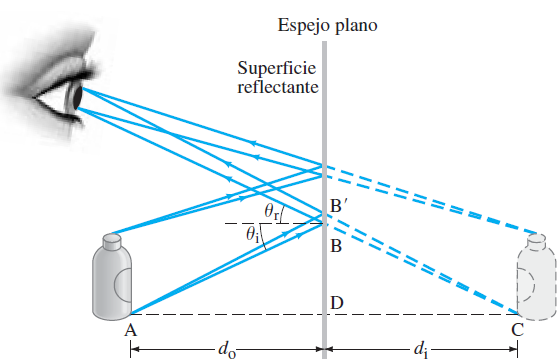
\includegraphics[width=0.6\textwidth]{images/espejo_plano.png}
	\caption{Espejo plano reflejando una botella. Se marcan los rayos que ingresan al ojo.}
	\label{fig:esplejos_planos}
\end{figure}

También se puede observar una \textbf{inversión en profundidad}, por ejemplo, la mano derecha reflejada parece la izquierda. Esto puede entenderse como un cambio en la orientación del sistema de coordenadas: si en un sistema cartesiano $\hat{i} \times \hat{j} = \hat{k}$, al reflejarse, se convierte en $\hat{i} \times \hat{j} = -\hat{k}$.

\begin{figure}[H]
	\centering
	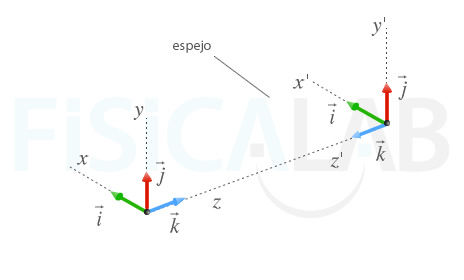
\includegraphics[width=0.6\textwidth]{images/inversion_profundidad.jpg}
	\caption{Inversión de profundidad en espejos planos.}
	\label{fig:inversion_profundidad}
\end{figure}

\subsubsection*{Espejos Esféricos}

En la figura \ref{fig:espejo_esferico}, un haz de rayos provenientes del punto $P$ sobre el eje óptico incide sobre un espejo esférico cóncavo y converge en el punto $P'$, conocido como \textbf{imagen real}, ya que la luz realmente pasa por ese punto. Esta imagen puede ser observada directamente.

\begin{figure}[H]
	\centering
	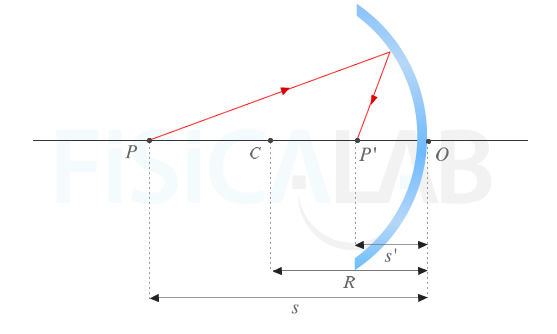
\includegraphics[width=0.6\textwidth]{images/espejo_esferico_AV.jpg}
	\caption{Los rayos provenientes del punto $P$ se reflejan en el espejo cóncavo y convergen en $P'$.}
	\label{fig:espejo_esferico}
\end{figure}

Cuando los rayos reflejados se alejan del eje, pueden producirse \textbf{aberraciones esféricas}, ya que no convergen exactamente en el mismo punto.

Para relacionar $P$ y $P'$, se utiliza la geometría óptica. En la figura \ref{fig:geometria_espejos_imagen} se puede deducir que:

\begin{equation}
	\alpha + \gamma = 2\beta
\end{equation}

\begin{figure}[H]
	\centering
	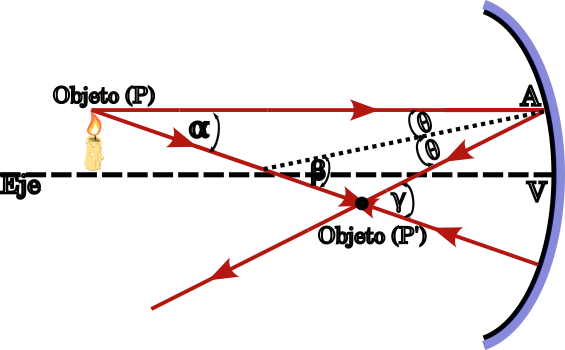
\includegraphics[width=0.6\textwidth]{images/geometria_espejos.png}
	\caption{Geometría de reflexión en espejos esféricos.}
	\label{fig:geometria_espejos_imagen}
\end{figure}

\subsubsection*{Fabricación de Espejos}

La fabricación de espejos requiere materiales pulidos con alta precisión, como vidrio con recubrimiento de aluminio o plata. El proceso varía según si el espejo es plano o curvo, y puede implicar técnicas como deposición por vacío o esmerilado óptico.

\subsection{Refracción y Lentes}

Cuando un objeto está parcialmente sumergido (por ejemplo, en agua), se observa un cambio en su forma aparente. Esto ocurre por la \textbf{refracción}: la luz cambia de dirección al pasar de un medio a otro, debido al cambio de velocidad de propagación.

Como se definió antes, el índice de refracción es:

\begin{equation}
	n = \frac{c}{v}
	\label{eq:indice_refraccion}
\end{equation}

Por ejemplo: aire $\approx 1.003$, agua $= 1.33$, vidrio $= 1.5$.

Cuando la luz pasa de un medio menos denso a uno más denso ($n_1 < n_2$), se acerca a la normal. Si va del agua al aire ($n_1 > n_2$), se aleja de la normal.

\begin{figure}[ht]
	\centering
	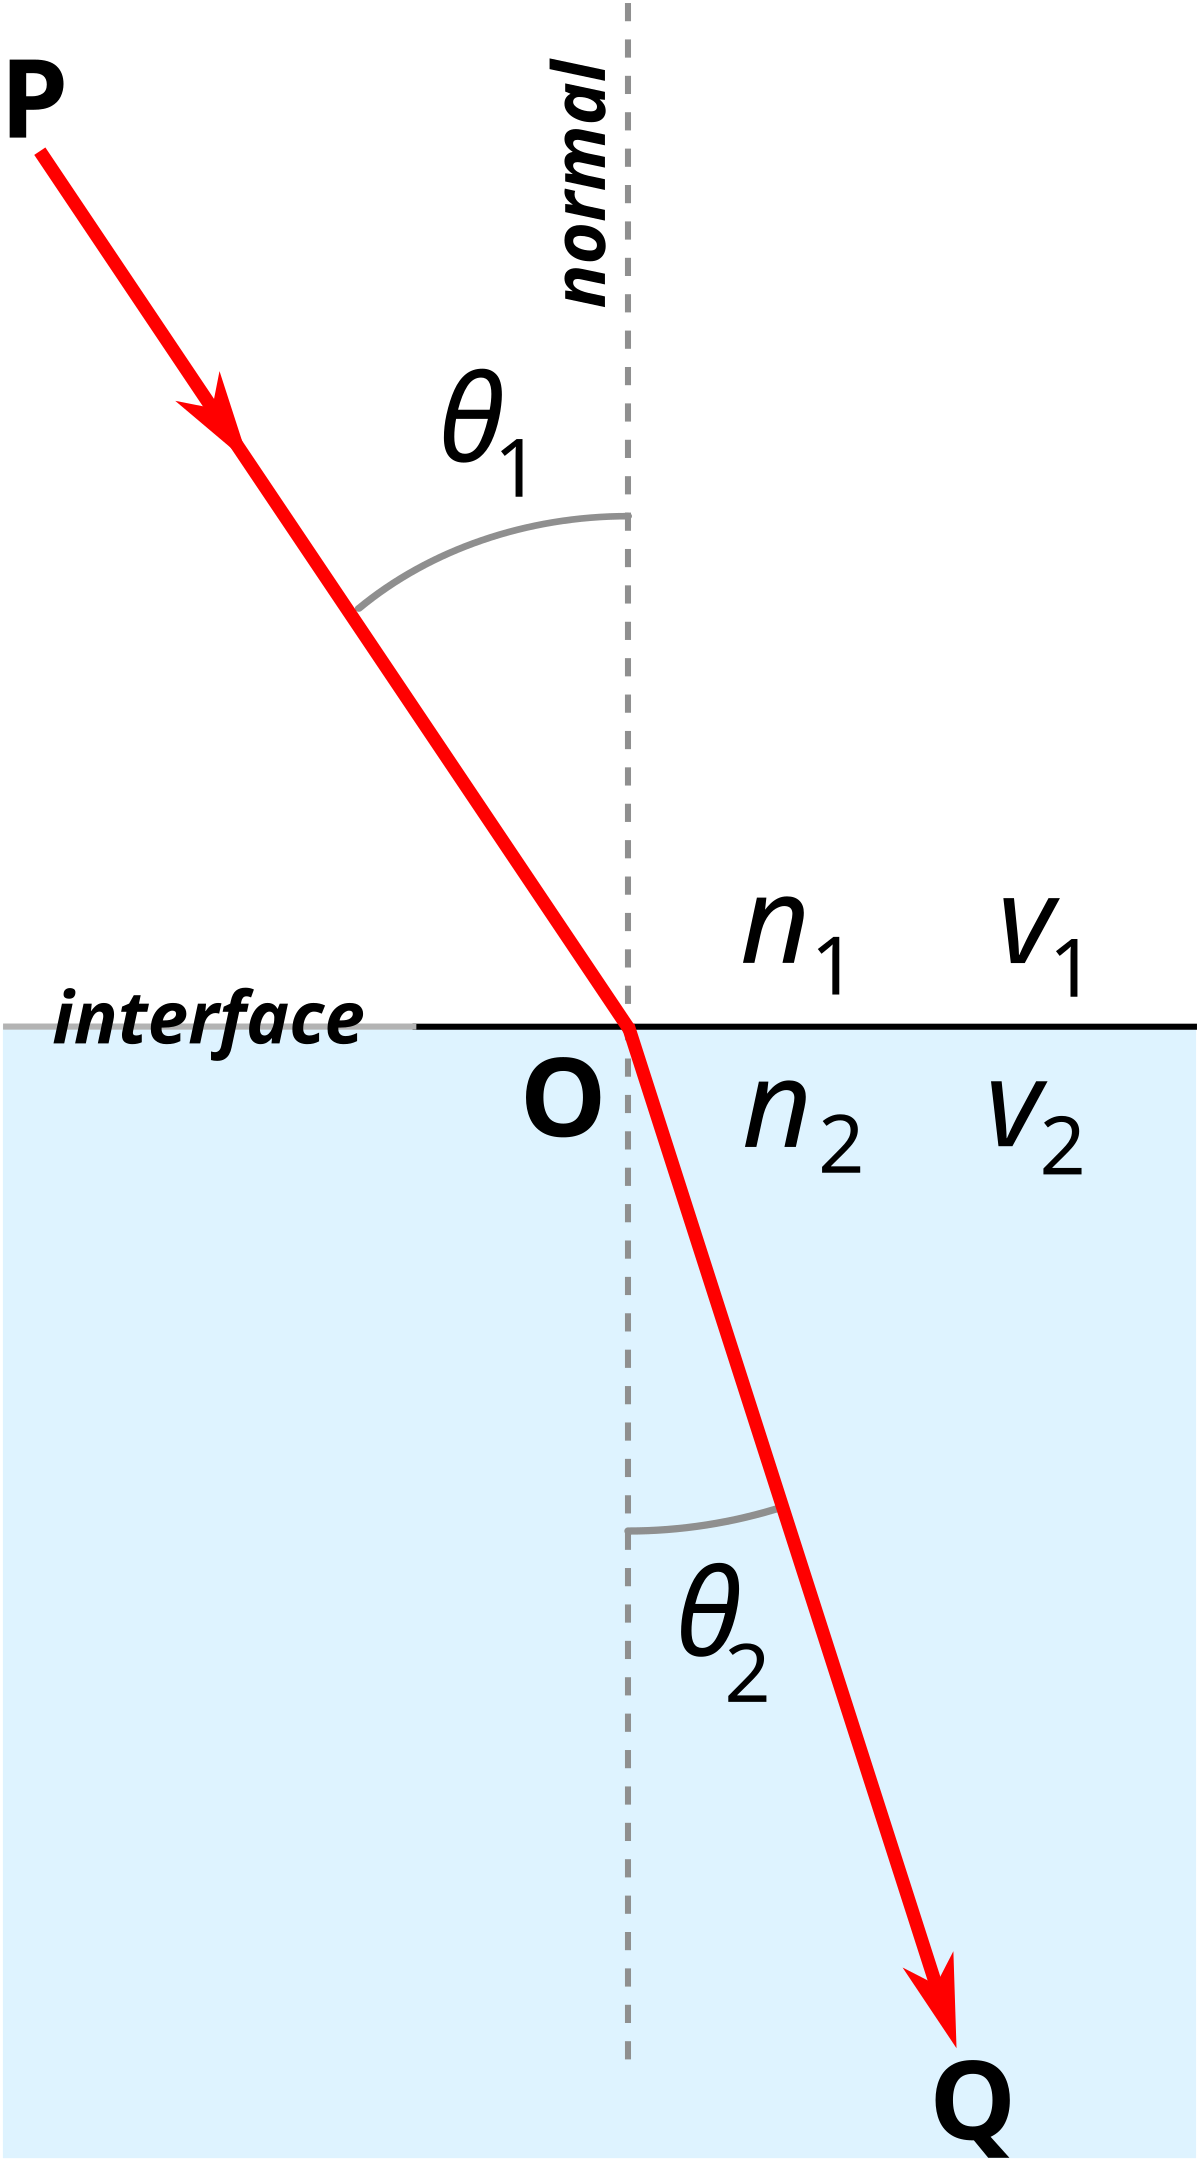
\includegraphics[width=0.5\textwidth]{images/Snells_law2.png}
	\caption{Refracción de la luz en una interfaz entre dos medios.}
	\label{fig:snell_law}
\end{figure}

Este cambio de dirección también se explica por el \textbf{Principio de Fermat}: la luz siempre sigue el camino óptico que le toma menos tiempo. Esta distancia efectiva se llama \textbf{camino óptico} y se calcula como $nd$.

Un caso especial ocurre cuando la luz pasa de un medio


\section{Tipos de Telescopios}

Como se mencionó al inicio, la palabra \textbf{telescopio} hace referencia a una serie de instrumentos, no únicamente al telescopio óptico, aunque comúnmente se asocie a él. Etimológicamente, el término implica “ver a lo lejos”, pero esto va más allá de la percepción visual humana. Los telescopios también abarcan regiones del espectro electromagnético que están fuera del rango visible.

Existen radiotelescopios, especializados en detectar ondas de radio provenientes del espacio. También hay telescopios infrarrojos y ultravioletas, diseñados para estudiar distintas regiones del universo a frecuencias específicas, con objetivos científicos particulares.

\subsection{Telescopios Refractores}

\subsection{Telescopios Refractores}

Los telescopios refractores son instrumentos ópticos que utilizan una o varias lentes para formar imágenes de objetos distantes. Son el tipo más antiguo de telescopio y se caracterizan por su construcción sencilla, durabilidad y estabilidad. En este diseño, la luz entra por la parte frontal del tubo óptico y atraviesa una lente llamada \textbf{objetivo}, que la refracta y concentra hacia un punto focal.

\textbf{Partes principales de un telescopio refractor:}
\begin{itemize}
	\item \textbf{Lente objetivo:} generalmente convergente (convexa), situada en la parte frontal del tubo. Su función es recoger la luz de objetos lejanos y hacerla converger en el foco.
	\item \textbf{Tubo óptico:} estructura mecánica que mantiene alineadas las lentes, bloquea la luz no deseada y protege el sistema óptico.
	\item \textbf{Enfocador:} mecanismo que permite mover el ocular hacia adelante o hacia atrás para lograr una imagen nítida.
	\item \textbf{Ocular:} lente (o conjunto de lentes) que actúa como una lupa para ampliar la imagen formada por el objetivo.
	\item \textbf{Montura:} estructura que sostiene el tubo y permite apuntarlo en distintas direcciones.
\end{itemize}

\textbf{Formación de la imagen:} el objetivo forma una \textbf{imagen real, invertida y reducida} en su plano focal. El ocular se posiciona en ese plano y actúa como una lente de aumento, proporcionando una imagen virtual, derecha (en el caso del diseño galileano) o invertida (en el diseño kepleriano).

\textbf{Distancia focal:} es la distancia entre el centro óptico de la lente objetivo y su foco. La \textbf{longitud del telescopio} suele estar dada aproximadamente por la suma de las distancias focales del objetivo y del ocular, especialmente si están alineados coaxialmente.

\subsubsection*{Ecuación de lentes delgadas}

Para un sistema de lente delgada, la relación entre la posición del objeto $s$, la posición de la imagen $s'$, y la distancia focal $f$ está dada por:

\begin{equation}
	\frac{1}{s} + \frac{1}{s'} = \frac{1}{f}
	\label{eq:lente_delgada}
\end{equation}

Donde:
\begin{itemize}
	\item $s$ es la distancia del objeto a la lente,
	\item $s'$ es la distancia de la imagen a la lente,
	\item $f$ es la distancia focal de la lente.
\end{itemize}

En astronomía, los objetos observados están a distancias prácticamente infinitas, por lo que se puede asumir $s \to \infty$ y la ecuación se reduce a $s' \approx f$.

\subsubsection*{Aumento angular}

El aumento proporcionado por un telescopio refractor se define como:

\begin{equation}
	M = \frac{f_\text{objetivo}}{f_\text{ocular}}
	\label{eq:aumento_telescopio}
\end{equation}

Donde:
\begin{itemize}
	\item $f_\text{objetivo}$ es la distancia focal de la lente objetivo,
	\item $f_\text{ocular}$ es la distancia focal del ocular.
\end{itemize}

Este cociente indica cuántas veces se amplía el ángulo visual del objeto respecto a la observación a simple vista.

\subsubsection*{Aberraciones ópticas en telescopios refractores}

Existen dos tipos de aberraciones ópticas comunes en telescopios refractores: la \textbf{aberración cromática} y la \textbf{aberración esférica}.

\begin{itemize}
	\item \textbf{Aberración cromática:} se debe a que el índice de refracción de los materiales varía con la longitud de onda. Como resultado, cada color se enfoca a una distancia distinta, generando bordes coloreados e imágenes poco nítidas.
	
	\item \textbf{Aberración esférica:} ocurre cuando la lente tiene una forma esférica. Los rayos que pasan por zonas más alejadas del eje óptico no convergen en el mismo punto que los rayos cercanos al eje, generando una imagen borrosa.
\end{itemize}

\subsubsection*{Corrección de aberraciones: lentes acromáticas}

Para reducir estas aberraciones, los telescopios modernos utilizan sistemas ópticos compuestos. Las \textbf{lentes acromáticas} son dobletes cementados compuestos por dos tipos de vidrio:

\begin{itemize}
	\item \textbf{Vidrio de corona:} bajo índice de refracción y baja dispersión.
	\item \textbf{Vidrio de pedernal:} alto índice de refracción y alta dispersión.
\end{itemize}

El diseño acromático permite que dos longitudes de onda (típicamente roja y azul) se enfoquen en un mismo plano, reduciendo significativamente la aberración cromática.

\textbf{Tipos de lentes acromáticas:}
\begin{itemize}
	\item \textbf{Doble acromático positivo:} una lente convergente de corona seguida por una lente divergente de pedernal.
	\item \textbf{Doble acromático negativo:} con combinaciones inversas, menos común.
	\item \textbf{Triplete acromático:} utiliza tres elementos para mejorar aún más la corrección de aberraciones.
	\item \textbf{Acromática asférica:} combina corrección cromática con superficie no esférica para minimizar también la aberración esférica.
\end{itemize}

Estos avances permiten que los telescopios refractores actuales generen imágenes de gran nitidez y fidelidad de color, manteniendo al mismo tiempo un diseño compacto y portátil.

\subsection{Telescopios Reflectores}

Los telescopios reflectores utilizan espejos curvados para formar imágenes, en lugar de lentes. Su diseño permite evitar ciertos problemas ópticos asociados con la refracción, como la aberración cromática. El primero de su tipo fue construido en 1668 por Isaac Newton, motivado por su descubrimiento de que la luz blanca se descompone en distintos colores al atravesar un prisma. Comprendió que al utilizar un espejo en lugar de una lente, se podía eliminar este efecto indeseado.

El \textbf{telescopio reflector newtoniano} original medía aproximadamente 15.5 cm de longitud y empleaba un espejo cóncavo de 4 cm de diámetro. La luz entraba por el extremo del tubo, se reflejaba en el espejo primario parabólico situado en el fondo, luego era redirigida por un espejo plano (diagonal) a 45° hacia un ocular ubicado en el lateral del tubo. Esta configuración permitió a Newton obtener una imagen nítida y sin dispersión cromática, con un rendimiento comparable al de telescopios refractores de más de un metro de longitud.

Décadas después, William Herschel desarrolló versiones mucho más grandes del diseño reflector. Comprendió que al incrementar el diámetro del espejo se podía captar más luz, lo que permitía observar objetos más tenues y lejanos. Gracias a esto, logró descubrir el planeta Urano en 1781. Su telescopio más famoso tenía un espejo de 1.2 metros de diámetro, construido con una aleación de cobre y estaño conocida como \textbf{metal de especulo}, que requería constantes repulidos debido a su rápida oxidación.

Hoy en día, los espejos se fabrican a partir de bloques de vidrio óptico (como Zerodur o Pyrex), que son fundidos y moldeados en hornos especiales. Luego se pulen con altísima precisión y se recubren con una fina capa de aluminio o plata, protegida por una película transparente que evita su degradación.

\subsubsection*{Partes principales de un telescopio reflector newtoniano}

\begin{itemize}
	\item \textbf{Espejo primario:} curvado (cóncavo), recoge la luz incidente y la enfoca en el plano focal. Puede ser parabólico o esférico.
	\item \textbf{Espejo secundario:} plano, montado en diagonal, redirige el haz de luz hacia el lateral del tubo.
	\item \textbf{Ocular:} lente (o conjunto de lentes) que amplifica la imagen formada por el espejo primario.
	\item \textbf{Tubo óptico:} mantiene la alineación entre los componentes y evita la entrada de luz no deseada.
	\item \textbf{Montura:} soporte que permite el movimiento y posicionamiento del tubo.
\end{itemize}

\subsubsection*{Principio óptico y formación de la imagen}

El funcionamiento de los telescopios reflectores se basa en la \textbf{ley de la reflexión}, la cual establece que el ángulo de incidencia es igual al ángulo de reflexión respecto a la normal en el punto de contacto:

\[
\theta_i = \theta_r
\]

Cuando la luz paralela proveniente de un objeto distante incide sobre un espejo cóncavo, esta se refleja y converge en el \textbf{foco}, formando una imagen real e invertida. Esta imagen es luego observada a través de un ocular, que amplía su tamaño aparente.

\subsubsection*{Ecuación del espejo esférico}

En la aproximación paraxial (rayos cercanos al eje óptico), la relación entre la distancia del objeto $s$, la distancia de la imagen $s'$, y la distancia focal $f$ del espejo esférico está dada por:

\begin{equation}
	\frac{1}{s} + \frac{1}{s'} = \frac{1}{f} = \frac{2}{R}
	\label{eq:espejo_esferico}
\end{equation}

Donde:
\begin{itemize}
	\item $s$ es la distancia del objeto al espejo (positiva si el objeto está frente al espejo),
	\item $s'$ es la distancia de la imagen al espejo (positiva si está en el mismo lado que el objeto),
	\item $f$ es la distancia focal,
	\item $R$ es el radio de curvatura del espejo ($f = R/2$).
\end{itemize}

\subsubsection*{Aumento lateral}

El aumento lateral describe el tamaño relativo de la imagen respecto al objeto:

\begin{equation}
	M = \frac{y'}{y} = -\frac{s'}{s}
	\label{eq:aumento_lateral}
\end{equation}

Donde:
\begin{itemize}
	\item $y$ es la altura del objeto,
	\item $y'$ es la altura de la imagen,
	\item $M > 0$ indica imagen derecha,
	\item $M < 0$ indica imagen invertida.
\end{itemize}

Cuando $|M| > 1$, la imagen está ampliada. Si $|M| < 1$, está reducida.

\subsection*{Fabricación de espejos}

Los primeros espejos utilizados en astronomía eran metálicos, principalmente de “metal de especulo”, que reflejaban la luz pero se degradaban rápidamente con la oxidación. Esto obligaba a repulir frecuentemente, lo cual afectaba la forma del espejo y su rendimiento.

Con el desarrollo de nuevos materiales, los espejos modernos se fabrican a partir de vidrio con bajo coeficiente de dilatación térmica (como Pyrex, Zerodur o borosilicato). Estos se funden en moldes precisos, se enfrían lentamente (proceso de recocido), y luego se pulen con extrema precisión (del orden de nanómetros). Finalmente, se recubren con una capa reflectante de aluminio o plata mediante deposición al vacío, y se sellan con una capa protectora para aumentar su durabilidad y resistencia ambiental.

Gracias a estas mejoras, los telescopios reflectores actuales son capaces de alcanzar aperturas superiores a los 10 metros y ofrecer imágenes de altísima resolución sin aberraciones cromáticas.


\subsection{Telescopios Catadióptricos}

Los telescopios catadióptricos son sistemas ópticos híbridos que combinan componentes \textbf{refractivos} (lentes) y \textbf{reflectivos} (espejos) para formar imágenes. Este diseño se aprovecha de las ventajas de ambos tipos de telescopios, reduciendo muchas de sus limitaciones ópticas y mecánicas.

El principio fundamental de los catadióptricos es el uso de una \textbf{lente correctora} en la parte frontal del tubo que modifica la trayectoria de los rayos antes de que estos lleguen a un \textbf{espejo primario curvado} (normalmente esférico). Posteriormente, la luz se refleja hacia un \textbf{espejo secundario}, y finalmente atraviesa un orificio en el centro del espejo primario para llegar al \textbf{ocular} o a un sensor ubicado en la parte trasera del telescopio.

\subsubsection*{Diseños más comunes}

\begin{itemize}
	\item \textbf{Schmidt-Cassegrain:} utiliza una delgada lámina correctora de Schmidt en la parte frontal y un espejo secundario convexo. Tiene un diseño cerrado y muy compacto.
	\item \textbf{Maksutov-Cassegrain:} emplea una lente correctora de menisco (más gruesa y robusta), que también ayuda a mantener la colimación del sistema. Presenta gran durabilidad mecánica y excelente calidad de imagen.
\end{itemize}

Ambos diseños logran una \textbf{gran distancia focal efectiva} en un tubo corto, gracias al plegado de la trayectoria óptica por reflexión interna. Esto permite observar con gran aumento sin necesidad de tubos largos, como en los refractores clásicos.

\subsubsection*{Partes principales de un telescopio catadióptrico}

\begin{itemize}
	\item \textbf{Lente correctora:} se encuentra en la parte frontal del tubo y corrige la aberración esférica introducida por el espejo primario.
	\item \textbf{Espejo primario:} cóncavo, de forma esférica, capta la luz y la refleja hacia el espejo secundario.
	\item \textbf{Espejo secundario:} convexo, refleja la luz hacia atrás a través de un orificio central en el espejo primario.
	\item \textbf{Focuser u ocular trasero:} amplifica la imagen para su observación.
	\item \textbf{Tubo óptico sellado:} protege los elementos ópticos del polvo y la humedad, manteniendo la colimación por más tiempo.
\end{itemize}

\subsubsection*{Ventajas del diseño catadióptrico}

\begin{itemize}
	\item Excelente corrección de aberraciones ópticas (cromática y esférica).
	\item Gran distancia focal en un tubo corto y portátil.
	\item Sistema cerrado que reduce mantenimiento y evita turbulencias internas.
	\item Versatilidad para astrofotografía, observación planetaria, cielo profundo y terrestre.
	\item Compatible con múltiples accesorios: cámaras, filtros, monturas motorizadas, entre otros.
\end{itemize}

\subsubsection*{Limitaciones}

\begin{itemize}
	\item El costo suele ser más elevado que los reflectores de apertura similar.
	\item Necesitan mayor tiempo de aclimatación térmica por su diseño cerrado.
	\item El espejo secundario obstruye parte del haz de luz (obstrucción central), lo cual reduce ligeramente el contraste en algunos casos.
\end{itemize}

\subsubsection*{Consideraciones prácticas}

Gracias a su equilibrio entre calidad óptica, portabilidad y facilidad de uso, los telescopios catadióptricos son muy populares entre astrónomos aficionados avanzados y observatorios escolares. Son ideales para quienes buscan un único instrumento versátil que funcione bien en múltiples contextos de observación.

\textbf{Resumen:} los telescopios catadióptricos integran en un solo sistema las fortalezas de los refractores y reflectores, proporcionando una solución óptica avanzada, compacta y versátil, ideal tanto para observación visual como para astrofotografía.
\section{Parámetros Clave de un Telescopio}

Los telescopios son instrumentos ópticos diseñados para captar y enfocar luz proveniente de objetos lejanos, permitiendo observar detalles invisibles al ojo humano. Para entender cómo se comporta un telescopio más allá de su tipo, es esencial conocer los parámetros físicos que definen su funcionamiento. Estos influyen directamente en el rendimiento óptico, la capacidad de observación y la utilidad del instrumento según su propósito (planetaria, cielo profundo, terrestre, etc.).

Los parámetros principales son: \textbf{apertura}, \textbf{distancia focal}, \textbf{relación focal}, \textbf{aumento}, \textbf{resolución angular}, \textbf{campo visual}, \textbf{magnitud límite}, \textbf{obstrucción central} y \textbf{tiempo de aclimatación térmica}.

\subsection{Apertura}
\label{subsec:apertura}

La \textbf{apertura} es el diámetro del objetivo (ya sea una lente o un espejo). Es el parámetro más importante del telescopio, ya que determina cuánta luz puede captar. Su impacto es doble:

\begin{itemize}
	\item \textbf{Captación de luz:} cuanto mayor sea la apertura, mayor es la cantidad de luz recogida, lo que permite observar objetos más débiles. La cantidad de luz captada es proporcional al área del objetivo ($\pi D^2/4$).
	\item \textbf{Resolución angular:} una mayor apertura reduce el tamaño del disco de difracción, permitiendo distinguir objetos muy cercanos entre sí (ver \ref{subse:aumento_resolucion}).
\end{itemize}

\textbf{Ejemplo:} un telescopio con una apertura de $70\,\mathrm{mm}$ capta aproximadamente 100 veces más luz que el ojo humano (apertura de $7\,\mathrm{mm}$).

\vspace{0.3cm}
\textbf{Insertar imagen sugerida:} Diagrama comparativo de aperturas con conos de luz y estrellas visibles.

\subsection{Distancia Focal}
\label{subsec:dist_focal}

La \textbf{distancia focal} $f$ es la distancia entre el objetivo (lente o espejo) y el punto donde convergen los rayos de luz paralelos al eje óptico. Para espejos cóncavos, se cumple:

\[
f = \frac{R}{2}
\]

donde $R$ es el radio de curvatura del espejo. En lentes delgadas, la distancia focal depende del índice de refracción y la curvatura:

\[
\frac{1}{f'} = (n - 1) \left( \frac{1}{R_1} - \frac{1}{R_2} \right)
\]

La distancia focal influye en:

\begin{itemize}
	\item El \textbf{aumento}: telescopios con distancia focal larga permiten mayor aumento para un mismo ocular.
	\item El \textbf{campo visual}: distancias focales más largas reducen el campo observable.
\end{itemize}

\vspace{0.3cm}
\textbf{Insertar imagen sugerida:} Rayos paralelos convergiendo en el foco en lente y espejo.

\subsection{Relación Focal (número f)}
\label{subsec:rel_focal}

La \textbf{relación focal} (número $f$) se define como:

\[
f/\# = \frac{f}{D}
\]

donde $f$ es la distancia focal y $D$ es la apertura del telescopio.

\begin{itemize}
	\item \textbf{Relaciones f bajas} ($f/4$ a $f/6$): óptimos para cielo profundo y astrofotografía (campo amplio, imagen brillante).
	\item \textbf{Relaciones f altas} ($f/10$ a $f/15$): ideales para observación planetaria (imagen más oscura, pero mayor aumento).
\end{itemize}

\subsection{Aumento}
\label{subse:aumento_resolucion}

El \textbf{aumento angular} ($M$) es la relación entre el tamaño angular de la imagen observada y el del objeto a simple vista:

\[
M = \frac{f_\text{obj}}{f_\text{ocular}}
\]

Donde $f_\text{obj}$ es la distancia focal del objetivo y $f_\text{ocular}$ la del ocular.

\begin{itemize}
	\item \textbf{Aumento mínimo útil:} 7x por cada centímetro de apertura.
	\item \textbf{Aumento máximo teórico:} 2x por milímetro de apertura (por ejemplo, $\sim200\times$ para un telescopio de 100 mm).
\end{itemize}

El aumento excesivo sin suficiente apertura resulta en imágenes borrosas y poco luminosas.

\subsection{Resolución Angular}

La \textbf{resolución} es la capacidad de distinguir dos objetos muy cercanos angularmente. Está limitada por la difracción y se calcula con el criterio de Rayleigh:

\[
\theta = 1.22 \cdot \frac{\lambda}{D}
\]

Donde:
\begin{itemize}
	\item $\lambda$ es la longitud de onda (en metros),
	\item $D$ es el diámetro de la apertura (en metros),
	\item $\theta$ es la resolución angular (en radianes).
\end{itemize}

También puede expresarse en segundos de arco:

\[
\text{Resolución (")} \approx \frac{138}{D\,\text{(mm)}}
\]

\vspace{0.3cm}
\textbf{Insertar imagen sugerida:} Diagrama de dos estrellas con disco de Airy, una resuelta y otra no.

\subsection{Campo Visual}

El \textbf{campo visual} (FOV) es el área del cielo observable a través del ocular. Depende de la distancia focal del telescopio y del ocular utilizado.

\[
\text{FOV aparente} = \frac{\text{AFOV del ocular}}{M}
\]

Donde $M$ es el aumento total. Oculares con mayor AFOV (apparent field of view) permiten observar más cielo.

\subsection{Magnitud Límite}

La \textbf{magnitud límite} es la magnitud aparente más débil que puede detectarse con un telescopio dado, dependiendo de la apertura. Se estima mediante:

\[
\text{Mag}_{\text{límite}} \approx 7.5 + 5 \cdot \log_{10}(D)
\]

con $D$ en milímetros. Por ejemplo, un telescopio de 100 mm puede alcanzar hasta la magnitud 12 aproximadamente.

\vspace{0.3cm}
\textbf{Insertar imagen sugerida:} Comparación visual entre campo observable con diferentes magnitudes.

\subsection{Obstrucción Central}

En telescopios reflectores y catadióptricos, el espejo secundario bloquea parte del haz de luz. Esta \textbf{obstrucción central} afecta el contraste de la imagen y la nitidez de los detalles finos. Se expresa como un porcentaje del diámetro total.

\subsection{Tiempo de Aclimatación Térmica}

Es el tiempo que requiere un telescopio para alcanzar el equilibrio térmico con el ambiente. Durante este tiempo, el tubo genera corrientes internas de aire caliente que degradan la calidad de la imagen. Los reflectores abiertos se aclimatan más rápido que los telescopios sellados como los catadióptricos.

---

\textbf{Resumen:}  
\begin{itemize}
	\item La \textbf{apertura} determina la captación de luz y la resolución.
	\item La \textbf{distancia focal} y la \textbf{relación focal} definen el aumento y el campo visual.
	\item La \textbf{resolución} marca la capacidad para distinguir detalles finos.
	\item La \textbf{magnitud límite} indica qué tan tenues pueden ser los objetos visibles.
	\item Otros factores como la \textbf{obstrucción}, el \textbf{campo visual} y la \textbf{aclimatación térmica} también deben considerarse.
\end{itemize}






\section{Monturas de Telescopios}
\label{sec:monturas_telescopios}

Un telescopio necesita una montura o soporte que le permita mantenerse estable y apuntar con precisión a los objetos celestes. Además, la montura es fundamental para compensar el movimiento aparente de los astros causado por la rotación de la Tierra.

Las monturas se clasifican principalmente por los ejes de movimiento que permiten. Los tres tipos principales son: \textbf{altazimutal}, \textbf{ecuatorial} y \textbf{Dobsoniana}. Cada una presenta ventajas particulares que las hacen más adecuadas para ciertos tipos de observación o uso.

La elección de una montura influye directamente en la facilidad de uso del telescopio, su portabilidad, precisión en el seguimiento y posibilidad de realizar astrofotografía.

\subsection{Montura Altazimutal}
\label{sec:montura_altazimutal}

La montura altazimutal, también llamada \textbf{altacimutal}, permite el movimiento del telescopio en dos ejes perpendiculares:

\begin{itemize}
	\item \textbf{Azimut:} movimiento horizontal (0° a 360°), que define la dirección sobre el horizonte.
	\item \textbf{Altura o elevación:} movimiento vertical desde el horizonte hasta el cenit (0° a 90°).
\end{itemize}

Ambos movimientos se refieren a la posición del observador, por lo tanto, esta montura usa un sistema de coordenadas local.

\textbf{Ventajas:}
\begin{itemize}
	\item Muy intuitiva y fácil de usar.
	\item Ideal para observación terrestre o astronómica casual.
	\item Montura ligera y económica.
\end{itemize}

\textbf{Desventajas:}
\begin{itemize}
	\item No permite seguir objetos celestes con un solo movimiento (requiere ajustes simultáneos en ambos ejes).
	\item No es adecuada para astrofotografía de larga exposición sin seguimiento motorizado complejo.
\end{itemize}

\vspace{0.3cm}
\textbf{Insertar imagen sugerida:} Diagrama de montura altazimutal con ejes marcados.

\subsection{Montura Ecuatorial}
\label{subsec:montura_ecuatorial}

La montura ecuatorial utiliza como referencia el sistema de coordenadas celestes. Está diseñada para que uno de sus ejes (el eje polar) se alinee paralelamente con el eje de rotación de la Tierra.

\begin{itemize}
	\item \textbf{Eje polar (ascensión recta, AR):} gira paralelamente al eje terrestre.
	\item \textbf{Eje de declinación (Dec):} gira perpendicular al eje polar, permitiendo desplazamientos hacia el norte o sur celeste.
\end{itemize}

\textbf{Ventajas:}
\begin{itemize}
	\item Permite seguimiento continuo de objetos celestes con un solo eje.
	\item Ideal para observación astronómica prolongada y astrofotografía.
	\item Se puede apuntar a coordenadas celestes específicas (AR y Dec).
\end{itemize}

\textbf{Desventajas:}
\begin{itemize}
	\item Requiere alineación previa con el polo celeste.
	\item Es más compleja y costosa que una montura altazimutal.
	\item Menos intuitiva para uso terrestre.
\end{itemize}

\vspace{0.3cm}
\textbf{Insertar imagen sugerida:} Diagrama de montura ecuatorial mostrando alineación al polo celeste.

\subsection{Montura Dobson}
\label{subsec:montura_dobson}

La \textbf{montura Dobsoniana} es una variante simplificada de la montura altazimutal, diseñada específicamente para telescopios reflectores de gran apertura. Fue popularizada por John Dobson en los años 60, quien buscaba un diseño accesible, estable y fácil de fabricar para fomentar la astronomía amateur.

Esta montura es mecánicamente muy sencilla: utiliza una base giratoria de madera o metal para el movimiento en azimut y apoyos en forma de “balancín” para el movimiento en altura. No requiere contrapesos ni piezas mecánicas complejas.

\textbf{Ventajas:}
\begin{itemize}
	\item Extremadamente estable y resistente a vibraciones.
	\item Muy económica, incluso para aperturas grandes (200 mm o más).
	\item Ideal para observación visual de cielo profundo desde cielos oscuros.
	\item Requiere poco mantenimiento.
\end{itemize}

\textbf{Desventajas:}
\begin{itemize}
	\item No permite seguimiento automático (a menos que se modifique).
	\item No está pensada para astrofotografía.
	\item Su gran tamaño puede dificultar el transporte en telescopios de gran apertura.
\end{itemize}

\vspace{0.3cm}
\textbf{Insertar imagen sugerida:} Foto o esquema de un telescopio Dobson con base giratoria de madera.

\subsection*{Resumen Comparativo}

\begin{table}[H]
	\centering
	\caption{Comparación de tipos de montura}
	\begin{tabular}{|l|c|c|c|}
		\hline
		\textbf{Característica} & \textbf{Altazimutal} & \textbf{Ecuatorial} & \textbf{Dobson} \\
		\hline
		Facilidad de uso        & Alta          & Media          & Alta \\
		Seguimiento automático  & No (excepto motorizado) & Sí           & No (sin modificación) \\
		Astrofotografía         & Limitada      & Excelente       & No recomendable \\
		Costo                   & Bajo          & Medio-Alto     & Muy bajo \\
		Portabilidad            & Alta          & Media          & Media-Baja \\
		Montaje y alineación    & Sencillo      & Requiere alineación polar & Muy sencillo \\
		Mejor uso               & Terrestre/astronómico casual & Astronomía/astrofotografía & Cielo profundo visual \\
		\hline
	\end{tabular}
\end{table}



\section{Grandes Telescopios y Futuro en Astronomía}

El estado del arte en el desarrollo de telescopios terrestres y espaciales ha transformado nuestra capacidad de observación del universo. En las últimas décadas, los avances en óptica, ingeniería de precisión, control adaptativo y computación han permitido construir instrumentos cada vez más potentes, capaces de capturar objetos extremadamente tenues y lejanos.

\subsection*{Telescopios terrestres}

Los telescopios más grandes de la actualidad se construyen sobre suelo firme, aprovechando cumbres elevadas con condiciones atmosféricas favorables y cielos despejados. En general, utilizan grandes espejos segmentados con mecanismos de ajuste milimétrico que permiten seguir objetos con precisión durante largos períodos.

\begin{itemize}
	\item \textbf{Gran Telescopio de Canarias (GTC)}: ubicado en La Palma, España, tiene un espejo primario de 10.4 metros compuesto por 36 segmentos hexagonales. Opera principalmente en el rango visible e infrarrojo cercano y es uno de los telescopios ópticos más grandes del mundo.
	
	\item \textbf{Observatorio W.M. Keck}: ubicado en Mauna Kea, Hawái, cuenta con dos telescopios gemelos de 10 metros de diámetro. Es ampliamente utilizado para la detección de exoplanetas, espectroscopía estelar y observación de objetos distantes.
	
	\item \textbf{Telescopio Binocular de Arizona (LBT)}: localizado en el Monte Graham, cuenta con dos espejos de 8.4 metros montados en paralelo, lo que le da una capacidad de recolección de luz superior a muchos telescopios individuales. Su estructura alcanza 600 toneladas y permite un control de los espejos a escala milimétrica. La luz que recolecta alcanza objetos a más de 13 mil millones de años luz de distancia.
	
	\item \textbf{Very Large Telescope (VLT)}: situado en el desierto de Atacama (Chile), está compuesto por cuatro telescopios principales de 8.2 metros y cuatro telescopios auxiliares móviles. Utiliza óptica adaptativa y puede operar en modo interferométrico para simular una apertura equivalente mucho mayor.
\end{itemize}

\subsection*{Nuevas generaciones de telescopios terrestres}

Uno de los proyectos más prometedores es el \textbf{Observatorio Vera C. Rubin}, también situado en Chile. Está diseñado para realizar el cartografiado más profundo y extenso del cielo nocturno. Contará con la cámara digital más grande jamás construida para astronomía, con 3200 megapíxeles, capaz de capturar imágenes con un campo de visión de 9.6 grados cuadrados —equivalente a 40 veces el tamaño aparente de la Luna llena en el cielo.

Otro hito importante será el \textbf{Extremely Large Telescope (ELT)}, en construcción en el Cerro Armazones (Chile). Tendrá un espejo primario de 39.3 metros de diámetro, compuesto por 798 segmentos hexagonales. Será el telescopio óptico e infrarrojo más grande jamás construido y permitirá estudiar atmósferas de exoplanetas, galaxias primordiales y pruebas de física fundamental.

\subsection*{Telescopios espaciales}

Aunque los telescopios terrestres han alcanzado enormes aperturas, la atmósfera terrestre sigue siendo un limitante en términos de turbulencia, absorción y difracción. Para superar estas barreras, se han lanzado al espacio instrumentos ópticos que operan en ausencia de atmósfera:

\begin{itemize}
	\item \textbf{Telescopio Espacial Hubble (HST)}: lanzado en 1990, posee un espejo de 2.4 metros y ha proporcionado imágenes de altísima resolución del universo, sin distorsión atmosférica.
	
	\item \textbf{Telescopio Espacial James Webb (JWST)}: lanzado en 2021, con un espejo de 6.5 metros recubierto de oro, es capaz de observar en el infrarrojo con una sensibilidad sin precedentes. Ha permitido detectar galaxias formadas apenas 300 millones de años después del Big Bang.
	
	\item \textbf{Nancy Grace Roman Space Telescope (antes WFIRST)}: programado para su lanzamiento en esta década, tendrá un campo de visión 100 veces mayor que el del Hubble, especializado en estudios de energía oscura, exoplanetas y cartografiado del cielo profundo.
\end{itemize}

\subsection*{Importancia de la apertura y la óptica moderna}

La capacidad de un telescopio para captar luz depende directamente de su apertura. Cuanto mayor es el diámetro del objetivo (lente o espejo), más luz puede recolectar y mayor es su poder de resolución. La construcción de telescopios cada vez más grandes ha sido clave para explorar los confines del universo observable.

Históricamente, William Herschel ya comprendió este principio. Construyó telescopios reflectores de gran tamaño, incluyendo uno de más de 6 metros de longitud, con el que descubrió el planeta Urano en 1781. Su enfoque en aumentar la apertura sentó las bases del diseño moderno de telescopios reflectores.

Hoy, los grandes telescopios utilizan espejos curvados debido a que son más livianos, estables y fáciles de fabricar que las lentes equivalentes. La óptica adaptativa, los sistemas computarizados de guiado y los espejos segmentados han permitido sortear las limitaciones físicas y logísticas de construir espejos monolíticos gigantes.

\subsection*{Futuro de la astronomía observacional}

Con el avance de nuevas generaciones de telescopios tanto en tierra como en el espacio, estamos entrando en una era de observación de altísima precisión. La sinergia entre telescopios ópticos, infrarrojos y de otras bandas (radio, rayos X) permitirá responder preguntas fundamentales sobre el origen del universo, la evolución de las galaxias, y la existencia de vida fuera de la Tierra.

Proyectos como el ELT, el Roman Telescope y misiones propuestas para la detección directa de exoplanetas habitables marcarán un antes y un después en la exploración del cosmos. El futuro de la astronomía observacional se sostiene sobre la base de la ingeniería extrema, la óptica de precisión, y la colaboración internacional.



\section{Consideraciones para la Elección de un Telescopio}
\label{sec:consideraciones_para_elegir_telescopio}

La elección de un telescopio debe realizarse considerando todos los parámetros discutidos previamente, así como el tipo de observación que se desea realizar (planetaria, cielo profundo, astrofotografía o terrestre). A continuación, se presentan los factores clave a tener en cuenta al momento de elegir un telescopio:

\subsection*{Tipo de Telescopio}

\begin{itemize}
	\item \textbf{Refractor:} utiliza lentes para formar la imagen. Son robustos y duraderos, ya que los elementos ópticos están sellados y protegidos. Requieren poco mantenimiento y son ideales para observación planetaria y lunar. Sin embargo, presentan aberración cromática y, a partir de ciertas aperturas, su fabricación se vuelve costosa.
	
	\item \textbf{Reflector:} utiliza espejos (Newtoniano, principalmente). Ofrecen aperturas mayores a menor costo, lo que los hace ideales para observar objetos de cielo profundo como galaxias y nebulosas. Requieren colimación periódica y sus componentes ópticos están más expuestos.
	
	\item \textbf{Catadióptrico:} combinación de lentes y espejos. Corrigen muchas aberraciones y ofrecen un buen equilibrio entre calidad óptica, portabilidad y versatilidad. Son más compactos, tienen lentes protegidas y requieren poco mantenimiento. Aptos para planetaria, cielo profundo e incluso astrofotografía.
\end{itemize}

\vspace{0.2cm}
\textbf{Insertar imagen sugerida:} Comparación visual de los tres tipos: ruta óptica, tamaño del tubo y campo de visión.

\subsection*{Apertura (Diámetro del objetivo)}
\label{subsec:consideracion_apertura}

La apertura determina cuánta luz puede captar el telescopio. Cuanto mayor sea, mejor será la visibilidad de objetos tenues y mayor la capacidad para distinguir detalles finos (resolución angular). Está directamente relacionada con el poder de resolución, como se explica en \ref{subsec:apertura} y \ref{subse:aumento_resolucion}.

\begin{equation}
	\text{Resolución (")} \approx \frac{138}{D \text{ (mm)}} \quad \text{ o } \quad R = 1.22 \cdot \frac{\lambda}{D}
\end{equation}

Una apertura mayor implica:
\begin{itemize}
	\item Mayor captación de luz.
	\item Mejor resolución (menor disco de difracción).
	\item Aumentos útiles más altos.
\end{itemize}

\subsection*{Distancia Focal}

La distancia focal es la distancia desde el objetivo al punto donde converge la luz. Este valor influye en el aumento del telescopio y en el campo visual. 

\begin{itemize}
	\item Focales largas ($f > 1000\,\text{mm}$): aumentos más altos, campo visual más estrecho.
	\item Focales cortas ($f < 700\,\text{mm}$): campo más amplio, útiles para cielo profundo y observación de grandes regiones del cielo.
\end{itemize}

\subsection*{Relación Focal}

La relación focal es el cociente entre la distancia focal y el diámetro de la apertura ($f/\#$). 

\[
f/\# = \frac{f}{D}
\]

\begin{itemize}
	\item $f/\# < 6$: telescopios rápidos, ideales para cielo profundo y astrofotografía.
	\item $f/\# > 8$: telescopios lentos, ideales para planetaria y observaciones de alto detalle.
\end{itemize}

\subsection*{Aumento}

El aumento se calcula como:

\[
M = \frac{f_\text{telescopio}}{f_\text{ocular}}
\]

Aunque es un parámetro comúnmente promocionado, no debe considerarse el más importante al inicio. Aumentos altos con poca apertura resultan en imágenes oscuras y con poco contraste. Lo ideal es trabajar en el rango útil de aumento según la apertura:

\begin{itemize}
	\item Mínimo útil: $\sim 7 \times$ por cada cm de apertura.
	\item Máximo útil: $\sim 2 \times$ por mm de apertura.
\end{itemize}

\subsection*{Montura}

La montura es tan importante como el tubo óptico. Debe ser estable, precisa y adecuada al tipo de uso:

\begin{itemize}
	\item \textbf{Altazimutal:} intuitiva, fácil de usar. Ideal para observación terrestre o astronómica casual. Ver sección \ref{sec:montura_altazimutal}.
	
	\item \textbf{Ecuatorial:} permite seguimiento celeste con un solo eje. Ideal para astrofotografía y seguimiento prolongado. Ver sección \ref{subsec:montura_ecuatorial}.
	
	\item \textbf{Dobson:} variante simplificada de la altazimutal. Estable y económica. Ideal para cielo profundo con telescopios reflectores grandes. Ver sección \ref{subsec:montura_dobson}.
\end{itemize}

---

\textbf{Conclusión:}  
La elección de un telescopio depende del equilibrio entre presupuesto, facilidad de uso, mantenimiento, tipo de observación y portabilidad. Un telescopio de apertura moderada (por ejemplo, 100–130 mm), con montura estable, es ideal para iniciarse en la observación astronómica. A partir de ahí, se puede escalar en complejidad y especialización según el tipo de observación deseada.

%
%\section{Preguntas y Discusión}
%
%
%
%*   ¿Cuáles son los **tres tipos principales de telescopios**?
%*   Describe cómo funciona un **telescopio refractor** y qué componentes utiliza.
%*   ¿Cuáles son algunas de las **ventajas y desventajas** de un telescopio refractor?
%*   ¿Qué es la **aberración cromática** y en qué tipo de telescopio es un problema común?
%*   Explica el funcionamiento de un **telescopio reflector** y menciona sus componentes principales.
%*   ¿Para qué tipo de observaciones son más apropiados los **telescopios reflectores**?
%*   ¿Qué es un **telescopio catadióptrico** y cómo combina diferentes elementos ópticos?
%*   ¿Cuáles son las **ventajas** de un telescopio catadióptrico?
%*   ¿Qué se entiende por la **apertura** de un telescopio y por qué es importante?
%*   ¿Cómo afecta una **mayor apertura** a la observación astronómica?
%*   ¿Qué es la **distancia focal** de un telescopio?
%*   ¿Cómo se relaciona la distancia focal con el **aumento** de un telescopio?
%*   ¿Qué es la **resolución óptica** o el poder de resolución de un telescopio?
%*   ¿Por qué es importante tener una buena **resolución** en un telescopio astronómico?
%*   ¿Cómo se puede calcular la **capacidad de resolución** de un telescopio según el criterio de Rayleigh?
%*   ¿Cómo se diferencia el criterio de Dawes del criterio de Rayleigh para calcular la resolución?
%*   ¿Qué es el **"seeing"** y cómo afecta a la capacidad de resolución de un telescopio terrestre?
%*   ¿Cuál es la función del **objetivo** en un telescopio?
%*   ¿Cuál es la función del **ocular** en un telescopio?
%*   ¿Qué se entiende por **ganancia de luz** en un telescopio?
%*   ¿Cómo se calcula la ganancia de luz de un telescopio?
%*   ¿Por qué los primeros telescopios utilizaban **lentes** y por qué ahora se prefieren los **espejos** en telescopios grandes?
%*   ¿Qué ventajas ofrecen los **espejos** sobre las lentes en la construcción de telescopios?
%*   ¿Cómo influyen los **efectos de la atmósfera terrestre** en la observación astronómica?
%*   ¿Qué son las **"ventanas de la atmósfera"** y por qué son importantes para la astronomía terrestre?
%*   ¿Por qué es costoso construir y mantener **observatorios astronómicos** en tierra?
%*   ¿Cuáles son algunas de las **ventajas de observar desde el espacio** en comparación con la observación terrestre?
%*   ¿Qué tipo de radiación electromagnética es mejor observar desde el **espacio**?
%*   ¿Quién fue **Galileo Galilei** y cuál fue su papel en la historia del telescopio?
%*   ¿Qué descubrimientos astronómicos importantes realizó **Galileo** con su telescopio?
%*   ¿Cuál fue la contribución de **Isaac Newton** al diseño del telescopio?
%*   ¿Qué es la **aberración cromática** y cómo la resolvió Newton en su diseño de telescopio?
%*   ¿Qué tipos de **monturas** se utilizan para los telescopios? (Aunque no se detalla en las fuentes, se menciona la montura ecuatorial).
%*   ¿Qué diferencia hay entre **reflexión** y **refracción** de la luz?
%*   ¿Qué es el **plano focal** de un telescopio?
%*   ¿Cómo se forma una **imagen** en un telescopio refractor?
%*   ¿Cómo se forma una **imagen** en un telescopio reflector?
%*   ¿Qué papel juega la **óptica geométrica** en la comprensión del funcionamiento de los telescopios?
%*   ¿Qué es la **difracción** y cómo limita la resolución de un telescopio?
%*   ¿Qué son los **discos de Airy** y cómo se relacionan con la resolución?
%*   ¿Por qué es importante la **calidad de las ópticas** (lentes o espejos) en un telescopio?
%*   ¿Qué consideraciones son importantes al **elegir un telescopio**? (Aunque esta pregunta es general, las fuentes proporcionan mucha información que influiría en la respuesta).
%
%Estas preguntas cubren una amplia gama de temas relacionados con los telescopios, desde sus tipos y principios ópticos hasta su historia y consideraciones prácticas.
